% Basic LaTeX template
\documentclass[11pt]{article}

% Page layout
\usepackage[margin=1in]{geometry}

% Common packages
\usepackage{graphicx}
\usepackage{booktabs}
\usepackage{amsmath,amssymb}
\usepackage{siunitx}
\usepackage[hidelinks]{hyperref}

% Metadata
\title{Your Title Here}
\author{Your Name}
\date{\\\today}

\begin{document}

\maketitle

\begin{abstract}
% Brief summary of the document.
\end{abstract}

\tableofcontents
\newpage

\section{Introduction}

Modern utility‑scale wind turbines convert atmospheric kinetic energy into electricity by extracting momentum from the flow using aerodynamic blades that drive a generator through a rotating shaft. This report presents modeling and analysis of the University of Minnesota’s Clipper Liberty C96 turbine in Rosemount, MN, with the dual objectives of quantifying aerodynamic performance and assessing structural integrity under representative operating conditions.

The analysis employs Blade Element Momentum (BEM) theory to compute thrust and power, evaluate the coefficients of power (\(C_P\)) and thrust (\(C_T\)), and explore operating trends via pitch optimization and a two‑dimensional sweep of pitch and tip‑speed ratio. Structural assessment focuses on tower response—deflection under distributed wind loading and nacelle thrust—plus static failure checks (Rankine, Tresca, von Mises) and fatigue using a Goodman diagram. The workflow is implemented in MATLAB (see `Master_Submittal.m`) using provided turbine and material data under steady‑state and linear‑elastic assumptions.

\section{Methods}
In order to analytically determine key performance metrics such as the coefficient of power and thrust under specific conditions and the structural durability of the wind turbine, a model based on various theoretical and computational approaches was developed. Important assumptions leading to numerically derived equations included the following: steady-state conditions, uniaxial stress, no aerodynamic interference between the blades, linear elastic material behavior, and a rigid nacelle region. The analysis was completed such that each blade was treated as an individual airfoil with geometric properties as defined in Figure (?)

\subsection{Aerodynamic Analysis}

To initially compute the coefficient of power and the coefficient of thrust based on a constant wind velocity of 10 meters per second, a rotational velocity of 14 revolutions per minute, and a pitch angle of 0 degrees, fundamental qualities in airfoil dynamics were considered. Beginning with the quantities of known values, the angular velocity was converted to radians per second and the tip-speed ratio was calculated using the following equations.
\begin{equation}
\lambda = \frac{\omega R}{V_\infty}, \qquad \omega = \frac{2\pi n}{60}
\label{eq:tsr_omega}
\end{equation}
where \(\lambda\) is the tip-speed ratio, \(\omega\) is rotor speed [rad/s], \(R\) is rotor radius, \(n\) is rotor speed [RPM], and \(V_\infty\) is the freestream wind speed.
The axial induction factor was taken to be equal to ⅓ and thus the angular induction factor was determined using the following equation.
\begin{equation}
\lambda_r = \lambda\, \frac{r}{R}
\label{eq:lambda_r}
\end{equation}
Assuming \(a=\tfrac{1}{3}\) (momentum limit), the tangential induction factor is
\begin{equation}
a' = -\tfrac{1}{2} + \tfrac{1}{2}\, \sqrt{\,1 + \tfrac{4}{\lambda_r^{2}}\, a(1-a)\,}\, .
\label{eq:aprime}
\end{equation}
Considering the local velocities on an axial and tangential basis, the inflow angle between the rotor plane and the relative wind velocity was determined using the following equation.
\begin{equation}
\phi = \tan^{-1}\!\left( \frac{1 - a}{(1 + a')\,\lambda_r} \right)
\label{eq:phi}
\end{equation}
The local angle of attack was then determined by subtracting the section twist angle and the section pitch angle from the inflow angle as follows. 
\begin{equation}
\alpha = \phi - (\theta + \beta)
\label{eq:alpha}
\end{equation}
where \(\theta\) is local geometric twist and \(\beta\) is the blade pitch angle.
Once the angle of attack was obtained, coefficients of lift and drag were determined using interpolations of airfoil performance data. Additionally, for circular sections, the drag coefficient was taken to be constant and the coefficient of lift was taken as zero representative of a circular cross-section in flow. The values of lift and drag coefficients were then resolved into normal and tangential components of coefficients of force as shown in the following equations.
\begin{equation}
 C_n = C_L\cos\phi + C_D\sin\phi, \qquad C_t = C_L\sin\phi - C_D\cos\phi
\label{eq:cn_ct}
\end{equation}
Differential elements of thrust, torque, and power were then calculated by the following
\begin{equation}
\mathrm{d}T = \tfrac{1}{2}\,\rho\,V_{\mathrm{rel}}^{2}\, c\, C_n
\label{eq:dT}
\end{equation}
\begin{equation}
\mathrm{d}Q = \tfrac{1}{2}\,\rho\,V_{\mathrm{rel}}^{2}\, c\, C_t\, r
\label{eq:dQ}
\end{equation}
\begin{equation}
\mathrm{d}P = \mathrm{d}Q\,\omega
\label{eq:dP}
\end{equation}
where \(\rho\) is air density and \(c\) is local chord length.
Integration along the blade was then performed to determine total thrust and torque forces as well as the power using the following equations.
\begin{equation}
 T = B \int_{r_\text{hub}}^{R} \! \mathrm{d}T\,\mathrm{d}r, \qquad P = B \int_{r_\text{hub}}^{R} \! \mathrm{d}Q\,\omega\,\mathrm{d}r
\label{eq:integrals}
\end{equation}
\begin{equation}
 C_P = \frac{P}{\tfrac{1}{2}\,\rho\,A\,V_\infty^{3}}, \qquad C_T = \frac{T}{\tfrac{1}{2}\,\rho\,A\,V_\infty^{2}}
\label{eq:cp_ct}
\end{equation}
with rotor swept area \(A = \pi R^{2}\) and number of blades \(B\).
Finally, using the value of the power and of the thrust, the coefficient of power and the coefficient of thrust were calculated using the following equations.
(see \eqref{eq:cp_ct}).

A similar process was then used to find the optimal pitch angle of a wind turbine blade that maximizes the power coefficient for a given wind velocity and tip speed ratio. Since the pitch angle affects the angle of attack, which in turn affects the coefficients of lift and drag, the angle of attack was recomputed at each pitch angle within a predetermined range of pitch angle values. Once the angle of attack associated with each pitch angle was determined, the same process as previously defined was performed numerically solving from the angle of attack, to values of life and drag coefficients, to normal and tangential force components, to the relative velocity, to the differential thrust, to the magnitude of power, and finally to the coefficient of power. Once the coefficients of power associated with varying pitch angles were determined, the optimal pitch angle was analyzed as the one which yielded the maximum coefficient of power. 

Furthermore, for the simultaneous optimization of both the pitch angle and the tip speed ratio for a specific wind speed, a  two-dimensional optimization was performed to determine the conditions which would maximize the wind turbine’s coefficient of power. The same forces, differentials, and coefficients were solved as previously defined at each combination of the pitch angle and tip speed ratio. By evaluating all pitch angle and tip speed ratio combinations, the pairing which yielded the highest coefficient of power was identified as the optimal operating condition.

Wind turbines present the possibility of producing more power than what they are rated for. To prevent such overloading, the blade pitch necessary to make sure not to over power the turbine between the rated and cut-out speed at a given wind speed was determined. Similarly as previously described, at each pitch angle in a given range,and at each possible tip speed ratio, the coefficient of power was determined. The solution progressed from the induction factors, to the angle of attack, to local coefficients of drag and lift, to normal and tangential force coefficients, to relative wind speed, to differential torque and power, which eventually led to the calculation of power and coefficient of power. The coefficient of power was converted to the total output power by the following equation.
\begin{equation}
P = C_P\,\left(\tfrac{1}{2}\,\rho\,A\,V_\infty^{3}\right)
\label{eq:P_from_CP}
\end{equation}
Finally, the minimum pitch angle which maintained a calculated power that did not exceed the rated power was selected as the required pitch angle setting.

\subsection{Structural Analysis}

A structural analysis was additionally performed to investigate the tower deflection, static failure, and fatigue of the wind turbine tower. The structural analysis to be defined was performed over two loading scenarios: maximum loading with primary wind direction and maximum loading with a secondary wind direction less than 180 degrees from the primary direction. The thrust force for each case was calculated using the previously defined calculations to define the load applied in the, assumed stiff,  nacelle region.

For the deflection analysis of the wind turbine tower, the tower was modeled as a cantilevered beam with a variable cross-section. The moment distribution was calculated via integration of the distributed load and thrust forces from each height to the top of the tower. The following equations were used.
% Atmospheric boundary layer wind profile and distributed drag
\begin{equation}
 U(z) = U_{\text{ref}}\left(\frac{z}{z_{\text{ref}}}\right)^{\epsilon}
\label{eq:wind_profile}
\end{equation}
\begin{equation}
 q(z) = \tfrac{1}{2}\,\rho\,C_D(z)\,D(z)\,U(z)^2
\label{eq:distributed_drag}
\end{equation}
% Shear and moment from distributed load q(z) (cantilever, z measured from base)
\begin{equation}
 \frac{\mathrm{d}V}{\mathrm{d}z} = -q(z), \qquad \frac{\mathrm{d}M}{\mathrm{d}z} = -V(z)
\label{eq:shear_moment}
\end{equation}
% Curvature, slope, and deflection (Euler–Bernoulli)
\begin{equation}
 \kappa(z) = \frac{M(z)}{E I(z)}, \qquad \theta(z) = \int_0^{z} \kappa(\xi)\,\mathrm{d}\xi, \qquad w(z) = \int_0^{z} \theta(\xi)\,\mathrm{d}\xi
\label{eq:deflection}
\end{equation}
% Include nacelle distributed load in nacelle region if applicable
\begin{equation}
 q_{\text{nacelle}}(z) = \begin{cases} \dfrac{F_{\text{thrust}}}{h_{\text{nacelle}}}, & z\in[z_{\text{tower}}, z_{\text{tower}}+h_{\text{nacelle}}] \\ 0, & \text{elsewhere} \end{cases}
\label{eq:nacelle_load}
\end{equation}

For the stress analysis of the beam, the bending stress at the base of the tower was calculated using the following equations.
% Bending stress at base (outer fiber)
\begin{equation}
 \sigma_b = \frac{M\,c}{I}
\label{eq:bending_stress}
\end{equation}
The principal stresses were then determined as follows.
% Principal and shear stresses for (approximately) uniaxial bending
\begin{equation}
 \sigma_1 = \sigma_b, \quad \sigma_2 = 0, \quad \tau_{\max} = \frac{\sigma_b}{2}
\label{eq:principal_stresses}
\end{equation}
The stress was additionally modified to reflect the second scenario of load such that the stress was modified by a directional factor according to the following equation.
The directional modification for the secondary wind case is applied by
\begin{equation}
 \sigma_{\text{case2}} = \sigma_{\text{case1}} \cos(\Delta \psi)
\label{eq:direction_factor}
\end{equation}
where \(\Delta\psi\) is the change in wind direction between cases.

For the static failure analysis of the wind turbine tower, three static failure theories were applied. The Maximum Normal Stress Theory was applied such that
\begin{equation}
 n_{\text{MNST}} = \frac{S_y}{\sigma_\text{max}}
\label{eq:mnst}
\end{equation}
The Maximum Shear Stress Theory was applied such that
\begin{equation}
 n_{\text{MSST}} = \frac{S_y}{\sigma_\text{max}}
\label{eq:msst}
\end{equation}
The Distortion Energy Theory was applied such that
\begin{equation}
 n_{\text{DET}} = \frac{S_y}{\sqrt{\sigma_\text{max}^{2} + 3\,\tau^{2}}}
\label{eq:det}
\end{equation}

For the fatigue analysis of the wind turbine tower, modified Goodman criteria were used with the mean and alternating stresses defined by the following.
% Mean and alternating stress for fatigue
\begin{equation}
 \sigma_m = \tfrac{1}{2}(\sigma_{\text{max}}+\sigma_{\text{min}}), \qquad \sigma_a = \tfrac{1}{2}|\sigma_{\text{max}}-\sigma_{\text{min}}|
\label{eq:mean_alt}
\end{equation}
The endurance limit, then, was calculated by the following equation.
\begin{equation}
 S_e = k_a\,k_b\,k_c\,k_d\,k_e\,k_f\,S'_e, \qquad S'_e = 0.5\,S_{ut}
\label{eq:Se}
\end{equation}
Finally, the fatigue safety factor was calculated as follows.
\begin{equation}
 n_G = \frac{1}{\dfrac{\sigma_a}{S_e} + \dfrac{\sigma_m}{S_{ut}}}
\label{eq:goodman}
\end{equation}

\section{Results & Discussion}
First, the coefficient of power and thrust were calculated for when the wind speed is 10 meters per second, the rotational velocity of the turbine is 14 revolutions per minute and the pitch angle of the blades is 0 degrees. Using a lumped analysis and assuming an ideal system, the best possible coefficient of power occurs when the axial induction factor is equal to ⅓ and this value is 0.5926. This is known as the Betz Limit. While the value of the axial induction factor used in this analysis is ⅓, a lumped analysis was not used. Instead, the power was calculated by using equations for the aerodynamic analysis. The maximum coefficient of power was calculated as 0.4224.
Using the same lumped analysis, the maximum coefficient of thrust occurs when the axial induction factor is ½ and this value is 1. Again, a lumped analysis was not used and instead the force on the blade was calculated using the equations for aerodynamic analysis.  The maximum coefficient of thrust was calculated to be 0.7041. 


Figure \ref{fig:cp_ct_vs_pitch} shows the coefficients of power and thrust of the wind turbine as a range of pitch angles are used. Adjusting the pitch angle is done to maximize the power output of the wind turbine based on the wind speed. The wind speed given for this analysis is 8 meters per second, which is slower than the speed given earlier, so the blades need to be pitched to maximize the surface area of the blade that is exposed to the wind. The goal is to maximize the coefficient of power and take the losses of the coefficient of thrust. 
Using the same methods used to solve for the coefficients as before, they are calculated again with a sweep of the pitch angle from -15 to 15 degrees. The given tip speed ratio is used to calculate the rotational velocity of the turbine. Then the equations for aerodynamic analysis are used to calculate the coefficients of power and thrust for each pitch angle. The sweep of the pitch angle changes the lift and drag forces acting on the blade, causing a change in the torque on the blade. The pitch angle with the maximum lift force to drag force ratio will have the most torque and in turn the most power. Changing the pitch angle also changes the swept area of the blade. Factoring in these changes, it was determined that for the given wind speed and tip speed ratio, the pitch angle with the maximum coefficient of power is -2 degrees. At this point the coefficient of power is 0.4464 and the coefficient of thrust is 0.7583.

As shown in Figure \ref{fig:cp_2d}, we determined the maximum coefficient of power over a sweep of both blade pitch angle and tip speed ratio for a given wind velocity. This was done with a range of pitch angle from -15 to 15 degrees, and a tip speed ratio of 8 to 13. Using the aerodynamic analysis equations, with a given wind speed of 6 meters per second, the two dimensional sweep resulted in a maximum coefficient of power of 1.3321, and this occurs at a pitch angle of -5 degrees and a tip speed ratio of 12.985. This coefficient of power is much higher than the Betz limit of 0.5926, and is also above 1, which is the absolute maximum value that this coefficient can have. The coefficient of power is the power output divided by the power input and it is impossible to output more power than what is put in. This happens because the model can predict the coefficient of power accurately for normal operating conditions, but in this case of low wind speed and high tip speed ratios, the assumptions made no longer hold. 
\begin{figure}[ht]
  \centering
  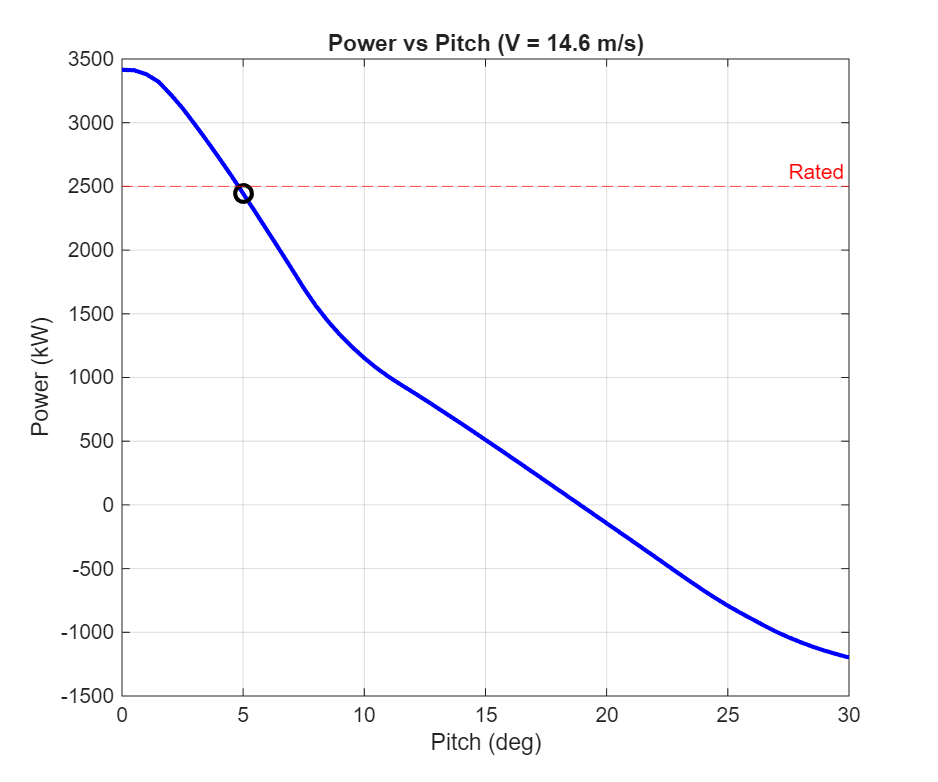
\includegraphics[width=0.9\textwidth]{Deliverable4_Power_vs_Pitch.png}
  \caption{Power vs. pitch angle at high wind speed with rated power line.}
  \label{fig:power_vs_pitch}
\end{figure}
Figure XXX: Plot of blade pitch angle needed to achieve rated power?
For a different wind speed of 14.6 meters per second, the pitch angle that gives the rated power output of 2.5 megawatts is found. This is done by calculating the worst case coefficient of power for each speed within the tip speed ratio for each pitch angle. Then the power is found using equation X. The minimum pitch angle where the power does not exceed the rated power is used as the ideal pitch angle, and it was found to be 4.9 degrees. As seen in Figure \ref{fig:power_vs_pitch}, any pitch angle below 4.9 degrees will result in a power higher than the rated power. If the power is above the rated value, this means the turbine is operating above the cut out speed. If this is sustained for a long time, this will result in mechanical failure of the turbine due to high stresses on it. This can also cause the electrical systems of the turbine to overheat and destroy the electrical components. 
\begin{figure}[ht]
  \centering
  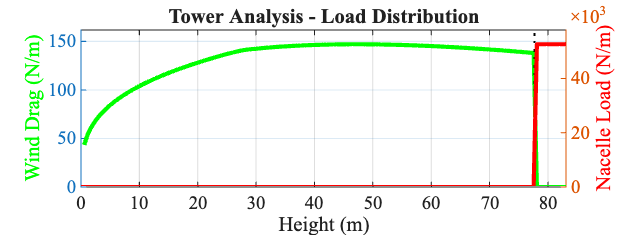
\includegraphics[width=\textwidth]{Tower_Load_Distribution.png}
  \caption{Distributed wind drag and nacelle load along height for both load cases.}
  \label{fig:tower_load_distribution}
\end{figure}
\begin{figure}[ht]
  \centering
  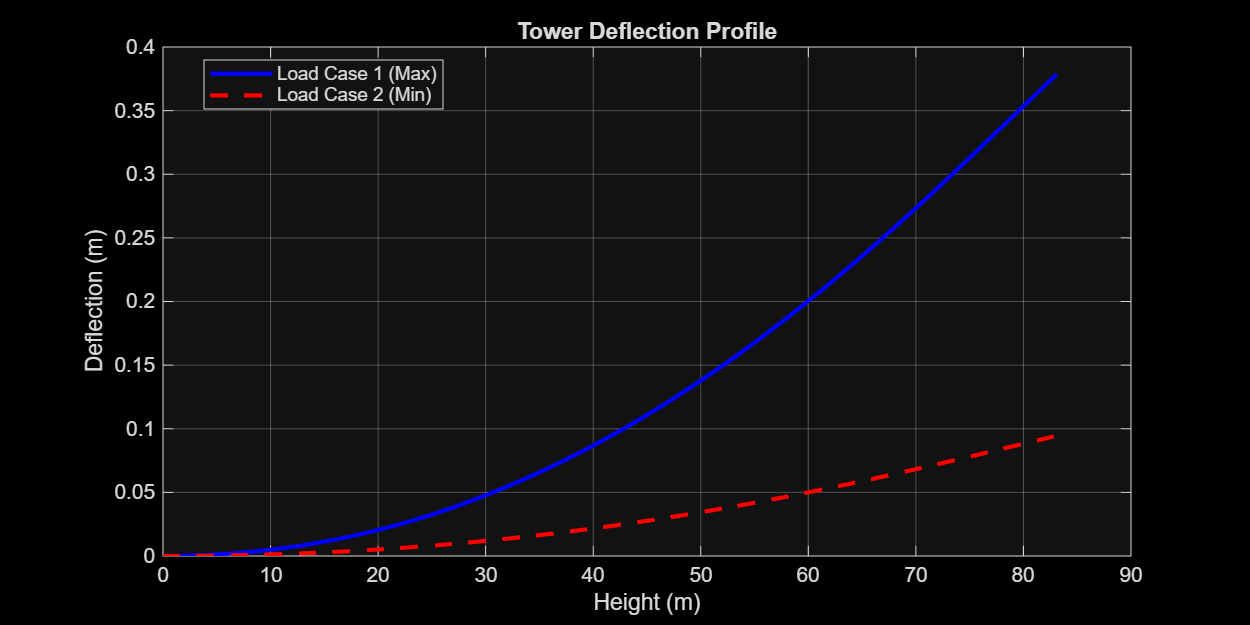
\includegraphics[width=\textwidth]{Tower_Deflection_Analysis.png}
  \caption{Tower shear, moment, slope, and deflection for both load cases.}
  \label{fig:tower_deflection}
\end{figure}
Lastly, a structural analysis of the wind turbine was performed, focusing on three aspects: deflection analysis, static failure analysis, and fatigue analysis. Determining the deflection of the tower was done by treating the tower as a cantilevered beam and using beam theory principles shown in equations X-X to solve for the load, shear, bending moment, slope and deflection at any point along the tower. The distributed load acting on the tower changes as a function of wind velocity and a power law exponent that changes based on the terrain roughness, resulting in a non constant load across the tower. The tower also has a non-constant cross sectional area and second moment of inertia. After using the beam theory principles, it was determined that the maximum deflection of the tower to be 0.383 meters. This deflection is around 0.25% of the height of the tower, which is well within the limits for the tower design. This deflection is well within the elastic deformation region, so there will not be any permanent damage to the wind turbine. For future analysis, the cone on the front of the turbine affects the thrust force acting on the blades, thus changing the distributed load acting on the blades. The thrust would become slightly larger, which would increase the distributed load on the nacelle, causing it to deflect slightly further. 
For static failure analysis, first the stresses of the tower are found. The only forces acting on the tower are the wind acting in the horizontal direction and the weight of the nacelle pushing axially on the tower. However, the bending stress applied on the tower from the wind dominates the axial force and causes it to have a very minor effect on the stress in the tower. Knowing this and general stress characteristics of a cantilevered beam, we know the maximum bending stress occurs at the ground. The location that the wind is in contact with experiences that stress in tension and on the other side of the tower it experiences compressive stress. This stress is calculated using equation X. Mohr’s Circle and equations X-X can be used to calculate the max stress and torque, knowing that there is no torque applied and the force only acts in one direction. Max stress was found to be Then using the max normal, max shear and distortion energy equations, the safety factor for each of these conditions is calculated using the yield stress of 345 megapascals per square inch. All three of these conditions give a safety factor of 8.11. This means that the highest stress exerted on the tower is approximately eight times lower than the ultimate tensile strength of the tower, which will allow for the tower to be able to handle much faster winds and more extreme conditions. Generally, the ideal safety factor for a wind turbine is 2, so with our safety factor of 8.11 we can conclude that the tower does not fail under static loading. 
For fatigue analysis, first the endurance limit of the material is calculated from the ultimate tensile strength of 450 megapascals using equation X. The constants in this equation are known and give an endurance limit of 148.75 megapascals. Then using equation X, the safety factor can be calculated from the known values of the alternating and mean stress in the part. The fatigue safety factor was found to be 3.418. This safety factor is also above 2, so we can conclude that the tower can safely operate in these conditions and not fail due to fatigue loading. Figure \ref{fig:goodman} shows the Goodman diagram, which is a visual representation of this fatigue loading case. The load line crosses the line of constant life first, so the safety factor can also be determined by dividing the length of the load line at the intersection with the line of constant life by the length of the load line at the operating point. 

\section{Conclusion}
Through the aerodynamic and structural analyses of a wind turbine, the performance and structural integrity of the turbine under various operating conditions were assessed. Quantitatively, a maximum coefficient of power of 0.4464 and a maximum coefficient of thrust of 0.7041 were determined for a set of prescribed conditions. Then a one dimensional optimization was performed, sweeping the pitch angle to determine the pitch angle with the best coefficient of power for a new set of operating conditions. It was determined that the ideal pitch angle is -2 degrees and it gives a coefficient of power of 0.4464. Next, a two dimensional optimization was performed that swept pitch angle and tip speed ratio with a different wind speed. The sweep was looking to find which combination of pitch angle and tip speed ratio gave the best coefficient of power, and it was determined that the model could not handle extreme operating conditions, with the coefficient of power being above the Betz Limit for high tip speed ratios. Additionally, the blade pitch necessary to ensure not to over power the turbine between the rated and cut-out speed at a wind velocity of 14.6 meters per second was determined to be 4.9 degrees requiring, then, that the blade pitch be kept under that angle at such higher wind speeds. Structurally, the tower deflection was determined to be 0.383 meters with safety factors of 8.11 for static failure and 3.418 for fatigue failure. With the deflection being within the limits for the tower design and both of the safety factors exceeding the ideal safety factor for a wind turbine, the tower was assessed to perform sufficiently under the defined conditions without being subjected to failure. 

Despite the clear successes based on the described model, limitations existed which could be improved upon for future analyses. Many assumptions were made which differ from a most ideal real-world representation of the wind turbine and the environment. Assumptions of steady-state flow and uniform wind velocity, for example, may be improved upon in future analyses via the incorporation of computational fluid dynamics to additionally model multi-dimensional, time-dependent flow. As for the structural analysis, one limitation of the model was the assumption of a rigid bodied nacelle. In future analyses, the implementation of a finite element analysis would allow for improved modeling of dynamic effects of the operating conditions.

Artificial intelligence was used to help troubleshoot bugs in the code, help give justifications and reasoning behind our results, and used to format the code block and plots output by the code.


% References (optional): If you have a .bib file, uncomment below
% \bibliographystyle{ieeetr}
% \bibliography{references}

\end{document}
